\begin{figure}
\begin{center}

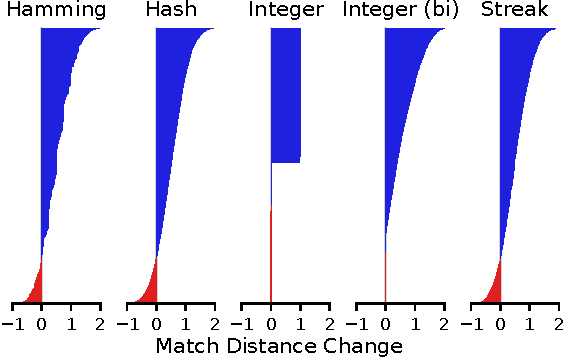
\includegraphics[width=\columnwidth]{{{detour_difference/bitweight=0dot5+seed=1+title=low-triplet-analysis+_data_hathash_hash=6b0749ef97a58721+_script_fullcat_hash=297c4fe09078e17b+ext=}}}
\caption{
Distributions of detour distance difference for triplets of randomly sampled tags.
Each bar sliver represents an independently sampled triplet A, B, and C.
A value of 2.0 indicates that the distance AC was zero and that the distances AB and BC were both 1.
A value of 0.0 indicates that the distance AC was equal to the distance AB plus AC.
A negative value (colored red) indicates violation of the triangle inequality: the distance AC is greater than the distance AB plus BC.
A value of -1.0 indicates the distance AC was equal to 1 but the distances AB and BC were both equal to zero.
}
\label{fig:detour_difference}

\end{center}
\end{figure}
